%!TEX root = ../dissertation.tex
\chapter{Implementation}

%\begin{figure}
%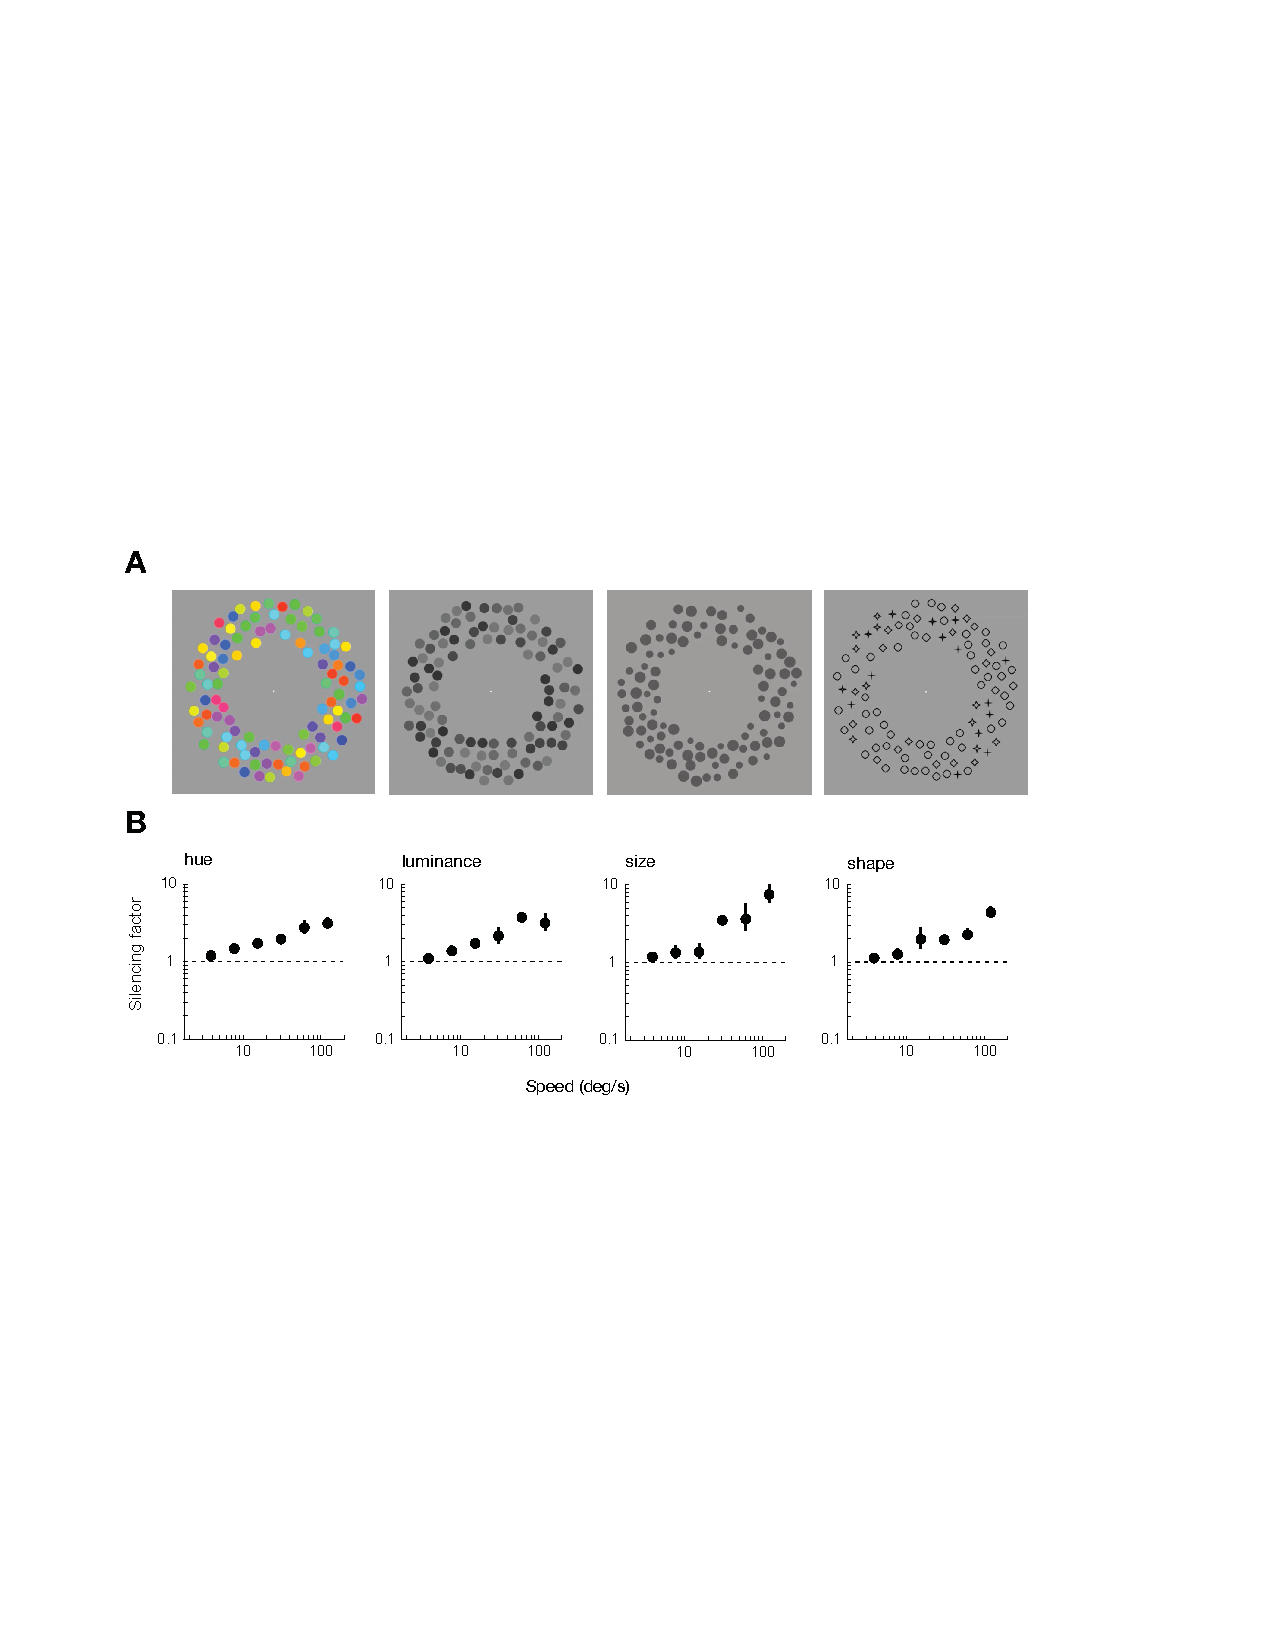
\includegraphics[width=\textwidth]{figures/fig1}
%\caption[Short figure name.]{This is a figure that floats inline and here is its caption.
%\label{fig:myInlineFigure}}
%\end{figure}

% For an example of a full page figure, see Fig.~\ref{fig:myFullPageFigure}.

%% Requires fltpage2 package
%%
% \begin{FPfigure}
% 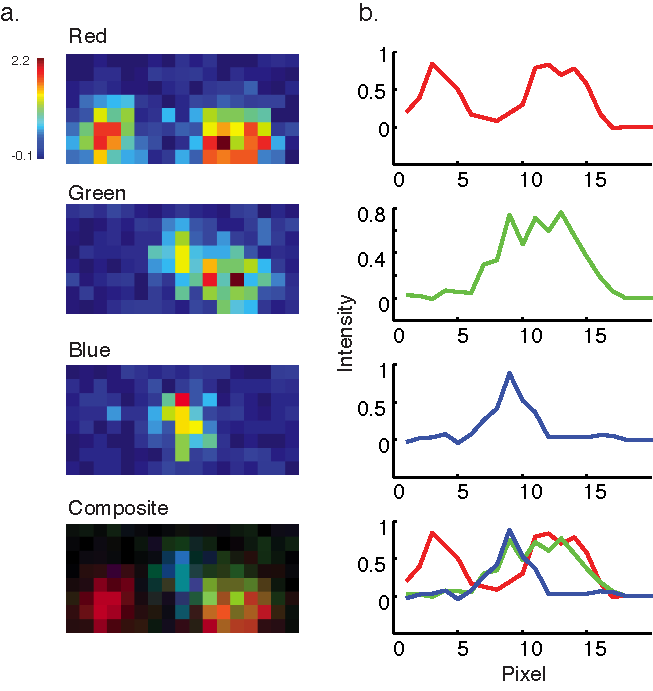
\includegraphics[width=\textwidth]{figures/fullpage}
% \caption[Short figure name.]{This is a full page figure using the FPfigure command. It takes up the whole page and the caption appears on the preceding page. Its useful for large figures. Harvard's rules about full page figures are tricky, but you don't have to worry about it because we took care of it for you. For example, the full figure is supposed to have a title in the same style as the caption but without the actual caption. The caption is supposed to appear alone on the preceding page with no other text. You do't have to worry about any of that. We have modified the fltpage package to make it work. This is a lengthy caption and it clearly would not fit on the same page as the figure. Note that you should only use the FPfigure command in instances where the figure really is too large. If the figure is small enough to fit by the caption than it does not produce the desired effect. Good luck with your thesis. I have to keep writing this to make the caption really long. LaTex is a lot of fun. You will enjoy working with it. Good luck on your post doctoral life! I am looking forward to mine. \label{fig:myFullPageFigure}}
% \end{FPfigure}
% \afterpage{\clearpage}

%\texttt{This is a line of code.}

\newthought{This chapter lays out the design and implementation} of the system used to generate optimal rule lists.
We begin by providing an overview of our algorithm.
Next, we explore the details of each of the three main data structures used to run our algorithm--a prefix trie, a symmetry-aware map, and a queue. 
We conclude with a more thorough walkthrough of the implementation of our main algorithm, including a discussion of our garbage collection and memory tracking.
%We conclude with a discussion of the garbage collection, design tradeoffs, and memory tracking framework used.

\section{Algorithm overview}
Our algorithm consists of 3 main steps.
First, we select the next rule list to evaluate.
Next, we evaluate the objective and bounds on this rule list and prune it if possible.
Finally, we update the optimal rule list if this rule list is better than the best rule list we have seen.
We continue with these 3 steps until we have no more prefixes to evaluate.
We provide a pseudocode version of our algorithm in Algorithm \ref{alg:branch-and-bound}.

\begin{algorithm}[t!]
  \caption{Branch-and-bound Algorithm for Rule Lists}
\label{alg:branch-and-bound}
\begin{algorithmic}
\normalsize
\State \textbf{Input:} A data set and a binary classification problem.\\
\State \textbf{Output:} Outputs the best rule list and its objective\\
\State Initialize data structures
\While {rule lists to examine}
	\State Get next rule list
	\State Evaluate rule list bounds, discard if possible
	\If {rule list is better than previous best}
		\State Update best rule list
		\State Garbage collection
	\EndIf
\EndWhile
\State \Return Best rule list, best objective
\end{algorithmic}
\end{algorithm}

\section{Prefix Trie}
%TODO Add picture of trie
The prefix trie is a custom C++ class and is used as a cache to keep track of rule lists we have already evaluated. 
Each node represents a rule---see Fig \ref{fig:cache_node} for our class definition of a node--and contains the id and prediction for the rule that the node represents.
Each leaf node in the trie contains the metadata associated with that corresponding rule list. 
This metadata includes the following bookkeeping information: viable child rule lists, lower bound, objective, minority misclassification, length, number captured, prediction for default rule, and whether or not this node should be pruned.
In addition to our base trie class, we implemented two different node types that we use in our algorithm.
First, we implemented a class that has an additional field that tracks the curiosity of a given prefix as defined in Section \ref{def:curiosity}.
Curiosity is one of several ways we use to order our search space.
Since the curiosity field is just a double, the memory overhead is minimal and the speed-up of using curiosity as opposed to BFS is sizable (see Section \ref{exp:priority}).
%We also implemented a class that has an additional field keeping track of the captured vector for that prefix.
%This captured vector has length $nsamples$, which means it is memory expensive.
%However, using the captured vector allows us to speed up our incremental computations because we would otherwise have to recompute this vector every time we used the prefix.

\begin{figure}[t!]
\begin{center}
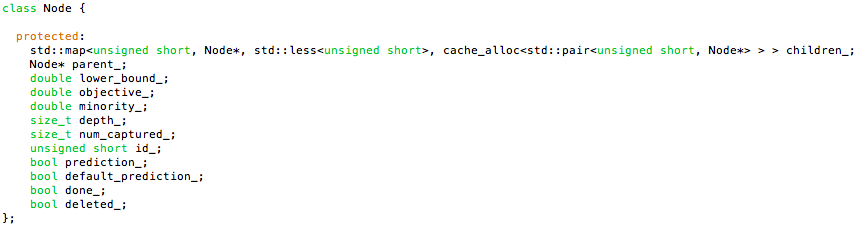
\includegraphics[width=\textwidth]{figs/cache_node.png}
\end{center}
\caption{Our custom C++ class defining a node in the prefix trie.}
\label{fig:cache_node}
\end{figure}

\section{Queue}\label{sec:queue}
%TODO fix this sentence
The queue is a worklist that orders which prefixes we are evaluating next.
Our queue support many different types of search policies that we use to explore the search space.
We implement a number of different scheduling schemes including BFS, DFS, various priority metrics, and a stochastic exploration process.
Our queue contains pointers to leaves in the trie to leverage incremental computation.
The search process involves selecting which leaf node to explore.
The stochastic exploration process bypasses the use of a queue by performing random walks on the trie until a leaf is reached.
Our other scheduling schemes use a STL C++ priority queue to hold and order all of the leaves of the trie that still need to be explored.
Our priority metrics can be ordered by curiosity, the objective, or the lower bound.
We find that using an exploitation strategy, such as ordering by curiosity or lower bound, usually leads to a faster runtime than using BFS.

In C++ the priority queue is a wrapper container that prevents access to the container underlying the queue.
Therefore we cannot access elements in the middle of the queue, even if we have know the value that we're trying to access..
Thus, we run into a problem where we may delete something in the prefix trie that is currently in the queue, as we have no way to update the queue without iterating over every element.
We address this by lazily marking nodes as deleted in the prefix trie without deleting the physical node until it has been removed from the queue.
As Fig \ref{fig:queue_gc} shows, this leads to a situation where our logical queue is actually smaller than the physical queue.

\begin{figure}[t!]
\begin{center}
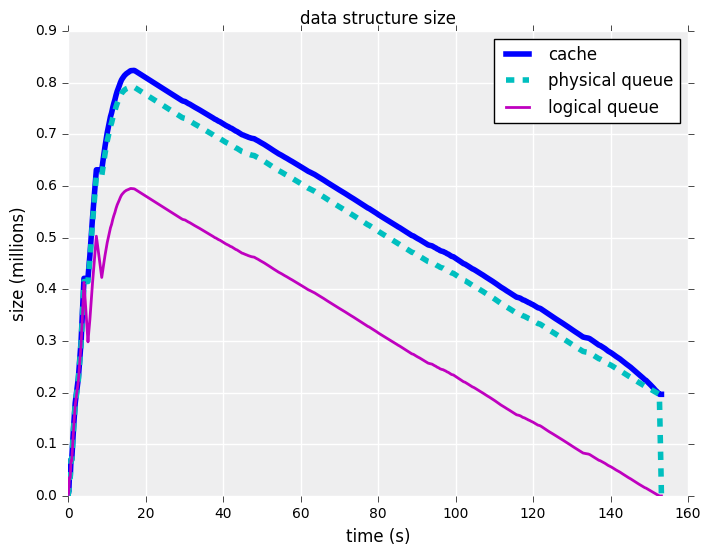
\includegraphics[width=0.9\textwidth]{figs/compas-queue-cache-size-insertions.png}
\end{center}
\caption{Size of prefix trie, logical queue, and physical queue over the execution of our algorithm on COMPAS data set.
This dataset has 155 rules and 6489 samples (see Section \ref{def:datasets}).
The gap between the logical queue and the physical queue is due to our lazy garbage collection}
\label{fig:queue_gc}
\end{figure}

\section{Symmetry-aware map}
We implement our symmetry-aware map as an STL unordered\_map, to apply the permutation bound described in Section \ref{def:perm-bound}.
We have two different versions of the map with different key types that allow permutations to be compared and pruned.
In both cases, the values consist of the best lower bound and the actual ordering of the rules that is best for that permutation.
In the first version, keys to the map are represented as the canonical order of the rules.
The second version has keys that represent the captured vector.
Our permutation is was based on the fact that different permutations capture the same data, so this type of key is equivalent for the rule lists (1, 4) and (4, 1).
Representing keys with captured vectors could potentially match more permutations since two prefixes may not be permutations of each other but might capture the same data points and therefore fall under the permutation bound.
In fact, we find that this occurs only rarely, as the number of rule lists examined is only slightly less in the captured vector case.
Despite supporting only one bound, the permutation map plays a significant role in our memory usage.

%TODO Refer to this figure or move elsewhere
\begin{figure}[t!]
\begin{center}
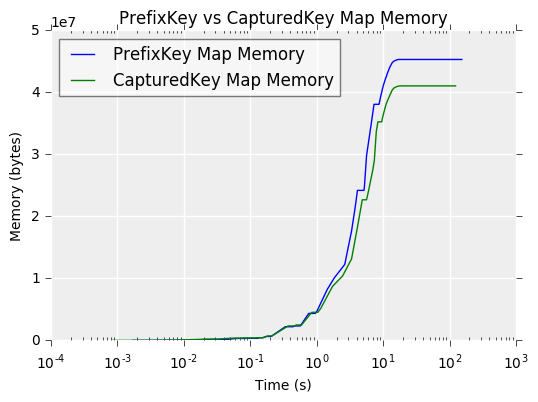
\includegraphics[width=0.9\textwidth]{figs/prefix-captured_pmap_mem.png}
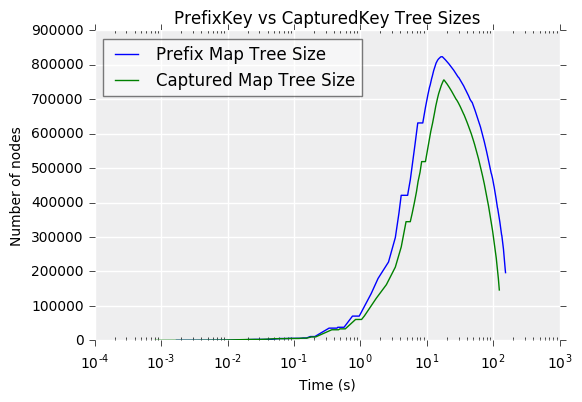
\includegraphics[width=0.9\textwidth]{figs/prefix-captured_tree_size.png}
\end{center}
\caption{This graph shows the memory usage of the map when using CapturedKeys and PrefixKeys. 
We see that CapturedKeys provide minimal space savings over PrefixKeys due to the slight decrease in nodes inserted into the trie.}
\label{fig:prefix-captured}
\end{figure}


\section{Incremental execution}
Our program terminates when all leaves of the trie have been explored and there is nothing else in our queue.
We can also opt for early termination based on the number of leaves in the trie.
This prevents us from achieving the certificate of optimality, but can still lead to us finding a good or even optimal rule list.
Most executions find the optimal rule list quickly, but then certification requires a long time and a large amount of memory.
Early termination allows us to trade the guarantee of optimality for lower time and memory costs.
%choose to not receive the full certificate of optimality by exiting execution when a certain number of rule lists are in the trie.
While there are still leaves of the trie to be explored, we use our scheduling policy to select the next rule list to evaluate.
Then, for every rule that is not already in this rule list, i.e. that we could potentially add to the list, we calculate the lower bound, objective, and all of the metrics shown in Fig \ref{fig:cache_node}.
We check the support bounds, the hierarchal objective bound, the permutation bound, and the lookahead bound.
If the new rule list has a lower bound that is better than all of these bounds, only then do we insert it into the permutation map, the prefix tree, and the queue, updating the minimum objective if necessary.
Otherwise, we do not insert it into any of our data structures, and we continue to the next potential rule, having excluded a rule list from being optimal.
After evaluating all the rules we could add to the current rule list, we return to the main loop and examine the next element in the queue.

\begin{comment}
\begin{table}
\begin{subalgorithm}{.5\textwidth}
  \caption{Branch-and-bound Algorithm for Rule Lists}
\label{alg:branch-and-bound}
\begin{algorithmic}
\normalsize
\State \textbf{Input:} A data set and a binary classification problem.
\State \textbf{Output:} Outputs the best rule list and its objective\\
\State Initialize data structures\\
\While {rule lists to examine}
	\State Get next rule list
	\State Evaluate rule list bounds, discard if possible
	\If {rule list is better than previous best}
		\State Update best rule list
		\State Garbage collection
	\EndIf
\EndWhile
\State \Return Best rule list, best objective
\end{algorithmic}
\end{subalgorithm}
\begin{subalgorithm}{.5\textwidth}
  \caption{CORELS}
\label{alg:corels}
\begin{algorithmic}
\normalsize
\State \textbf{Input:} A data set and a binary classification problem.
\State \textbf{Output:} Outputs the best rule list and its objective.
\State $opt \gets NULL$
\State $T \gets initializeTree()$
\State $Q \gets queue(\,[T.root()\,])$
\State $P \gets map(\{\})$
\While {$Q$ not empty}
	\State $node \gets Q$.pop(\,)
	\State $newObj \gets$ incremental($node, T, Q, P$) \Comment{Defined below}
	\If {$newObj$ < $T$.minObjective(\,)}
		\State $opt \gets T$.bestRuleList(\,)
		\State $T$.garbageCollect(\,)
	\EndIf
\EndWhile
\State \Return $opt, T$.minObjective(\,)
\end{algorithmic}
\end{subalgorithm}
\end{table}
\end{comment}

%TODO refer to this
\begin{algorithm}[t!]
  \caption{CORELS}
\label{alg:corels}
\begin{algorithmic}
\normalsize
\State \textbf{Input:} A data set and a binary classification problem.\\
\State \textbf{Output:} Outputs the best rule list and its objective.\\
\State $opt \gets NULL$
\State $T \gets initializeTree()$
\State $Q \gets queue(\,[T.root()\,])$
\State $P \gets map(\{\})$
\While {$Q$ not empty}
	\State $node \gets Q$.pop(\,)
	\State $newObj \gets$ incremental($node, T, Q, P$) \Comment{Defined below}
	\If {$newObj$ < $T$.minObjective(\,)}
		\State $opt \gets T$.bestRuleList(\,)
		\State $T$.garbageCollect(\,)
	\EndIf
\EndWhile
\State \Return $opt, T$.minObjective(\,)
\end{algorithmic}
\end{algorithm}

\begin{comment}
\begin{algorithm}[t!]
  \caption{Branch-and-bound Algorithm for Rule Lists}
\label{alg:branch-and-bound}
\begin{algorithmic}
\normalsize
\State \textbf{Input:} A data set and a binary classification problem.\\
\State \textbf{Output:} Outputs the best rule list and its objective\\
\State Initialize data structures
\While {rule lists to examine}
	\State Get next rule list
	\State Evaluate rule list bounds, discard if possible
	\If rule list is better than previous best
		\State Update best rule list
		\State Garbage collection
	\EndIf
\EndWhile
\State \Return Best rule list, best objective
\end{algorithmic}
\end{algorithm}
\end{comment}

%TODO refer to this, and clean it up
\begin{algorithm}[t!]
  \caption{Incremental evaluation of a prefix}
\label{alg:incremental}
\begin{algorithmic}
\normalsize
\State \textbf{Input:} Node to be evaluated~$parent$,
prefix tree~$T$,
queue~$Q$,
symmetry-aware map~$P$
\State \textbf{Output:} None---destructively updates best objective in the tree\\
\State $prefix \gets parent$.prefix(\,)
\State $t \gets c *$ nsamples \Comment{This forms the threshold for our support bounds}
\For {$rule \notin prefix$}
	\State $rlist \gets prefix$.append($rule$)
	\State $cap \gets parent\text{.notCaptured(\,)} \wedge rule$.notCaptured(\,)
	\If {$|cap| < t$} \Comment{Minimum support bound}
		\State continue
	\EndIf
	\State $capZero \gets cap \wedge T$.zeroLabel(\,) \Comment{Record how many zeros the new rule captures}
	\State $corr \gets max\{|capZero|, |cap| - |capZero|\}$
	\If {$corr < threshold$} \Comment{Minimum correct support bound}
		\State continue
	\EndIf
	\State $lb = parent.\text{bound(\,)} - parent.\text{minority(\,)} + \frac{|cap| - corr}{nsamples} + c$ \Comment{Calculate lower bound}
	\If {$lb  >= T.$minObjective(\,)} \Comment{Objective bound}
		\State continue
	\EndIf
	\State $notCap \gets parent\text{.notCaptured(\,)} \wedge \neg cap$
	\State $notCapZero \gets notCap \wedge T$.zeroLabel(\,)
	\State $defaultCorr \gets max\{|notCapZero|, |notCap - notCapZero|\}$
	\State $obj \gets lb + \frac{|notCap| - defaultCorr}{nsamples}$ \Comment{Calculate objective}
	\If {$obj < T$.minObjective(\,)} \Comment{Update minimum objective}
		\State $T.minObjective(obj)$
	\EndIf
	\If{$lb + c >= T.$minObjective(\,)} \Comment{Lookahead bound---don't add to queue if its children will all be worse than the minimum objective}
		\State continue
	\EndIf
	\State $n \gets P.insert(rlist)$ \Comment{Symmetry-aware map handles permutation bound for us}
	\If {$n$} \Comment{$n$ will be NULL if it failed the permutation bound check}
		\State $T.$insert($n$)
		\State $Q.$push($n$)
	\EndIf
\EndFor
\end{algorithmic}
\end{algorithm}

\section{Garbage Collection}
Every time we update the minimum objective, we garbage collect the trie, by traversing from the root to the leaves.
Any time we encounter a node with a lower bound larger than the minimum objective, we delete its entire subtree.
In addition, if we encounter a node with no children, we prune upwards---deleting that node and recursively traversing the tree towards the root, deleting any childless nodes.
This garbage collection allows us to limit the memory usage of the trie.
In practice, though, the minimum objective is not updated that often, so garbage collection is triggered only rarely.

\section{Memory tracking}
Throughout our development of CORELS, we often ran into the problem that larger datasets would run us out of memory.
Therefore, we wanted to institute data structure optimizations that would reduce the memory burden of our algorithm.
In order to achieve this goal, we needed to implement a way of tracking how much memory our program was using and where it was being used.
We track memory through the use of C++11 custom allocators.
Our allocators are simple malloc wrappers that log which data structure the allocation is coming from--the trie, the map, or the queue.
We validated the accuracy of this memory tracking by running the program under Valgrind's Massif heap profiler tool and comparing the outputs.
Our outputs matched Valgrind's to within a few tenths of a percentage points, so we concluded that our memory tracking was successful.
On a limited run of the bcancer data set, Valgrind's tool Massif reported that we used 98.7 MB, while our data structure tracking recorded 98.5 MB, a difference of 0.2\% which is easily explained by miscellaneous heap allocations.
The heap profiling of Valgrind has a large overhead, while our memory logging has minimal overhead.
This allows us to output our memory usage per data structure on a regular basis without incurring the large overhead of Valgrind.